%
\chapter{Modeling \& Terminology}%
\label{chap:modeling}
As the design of humanoid robots is based on that of a human being, a lot of terms and models used by roboticists and human motion researchers overlap.  In this chapter, an overview is given of an important part of the fundamental naming and theory that is used for the system behavior and description of a humanoid robot. 
\section{Walking Terminology}
There are a variety of terms used in describing walking or locomotion. In this section, the terminology in this report is determined, which is also widely used, as for example can be found in \cite{charalambous2014walking}.
\subsection{Single support phase}
During the single support phase, the biped is only with one foot on the ground. The other foot is swinging through the air without ground contact, in the process of taking a step. The leg in contact with the ground is called the \textit{stance leg} and the leg taking a step is called the \textit{swing leg}. In a simplified walking model the single support phase with hybrid switching between contacts is often the only phase considered. There exist also bipedal robots with only this phase applied on hardware, like ATRIAS from Oregon State University \cite{ramezani2014performance}. This robot however, by the point-foot support with only the single stance leg per single support phase, has to keep stepping without interruption to stay stable, as the unstable equilibrium above the foot diverges quickly. 
\subsection{Double support phase}
In more human-like walking, next to the single support phase the double support phase is considered, also called the transfer phase in some cases. This is the phase during walking where both feet are on the ground.

\section{Full Robot Model}
The human body is a very complex system and has redundant joints and actuation. Among those joints exist joints with one degree of freedom, like the knee joint, but also joints with multiple degrees of freedom, like the hip joint for example. Reproducing this in robotics is a challenging task and different choices can be made in the complexity of the system and the type of actuators. 
\subsection{Current bipedal robots}
In \figref{fig:currentrobots} a couple of modern bipedal robots are displayed. \figref{fig:currentrobotsa} displays the newest model of Boston Dynamics' Atlas, a device that impressed a lot of people with its capabilities. It can run, stand up again after it has fallen over and it can even do a backflip, as shown in videos. Those are all incredible improvements with respect to earlier achieved results in humanoid robotics. \figref{fig:currentrobotsb} shows the previous Atlas model. This robot is used by IHMC to compete in the DARPA Robotics Challenge \cite{johnson2015team} and it gets still used to test new features on. \figref{fig:currentrobotsc} shows the Valkyrie humanoid robot \cite{radford2015valkyrie}, which is built by NASA. A version of this robot is also at IHMC. A difference between the Atlas robots and Valkyrie, is that the both Atlas versions are controlled with hydraulic actuation. Valkyrie makes use of so called series elastic actuators. \figref{fig:currentrobotsd} shows the ATRIAS robot from Oregon State University \cite{ramezani2014performance}. This is a good example of a, compared to the previous three examples, relatively more simple model. It has point feet and no arms for manipulation. In this report this is therefore defined as a bipedal robot, but not as a humanoid.
\begin{figure}[h]
  \begin{subfigure}{0.23\textwidth}
  \centering
  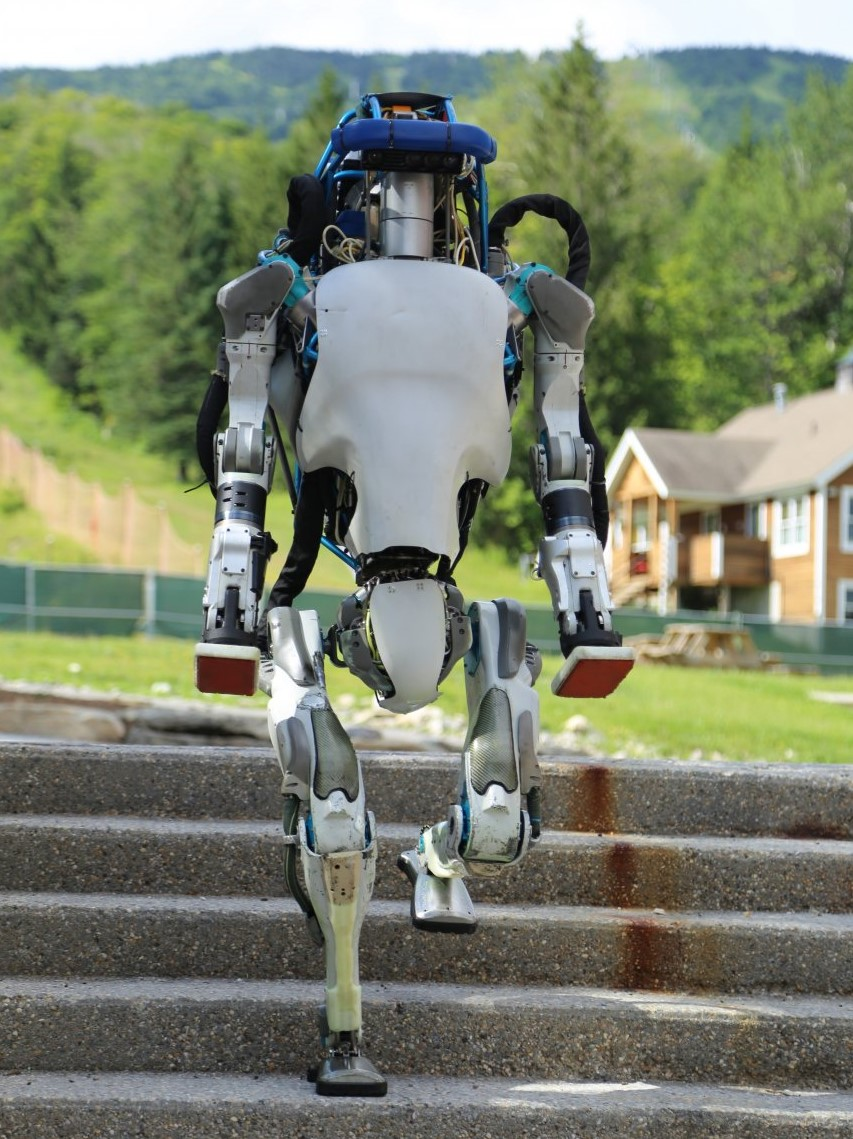
\includegraphics[width=.8\linewidth]{STYLESTUFF/AtlasNew.jpg}
   \caption{}
    \label{fig:currentrobotsa}
  \end{subfigure}
  \begin{subfigure}{0.23\textwidth}
    \centering
  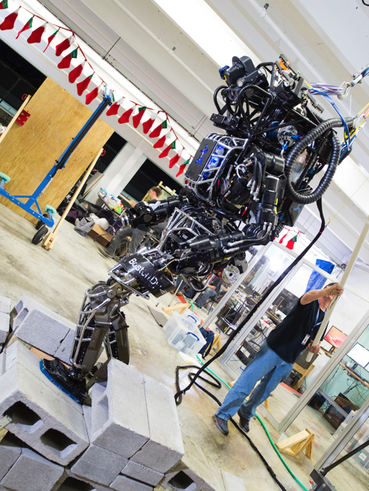
\includegraphics[width=.8\linewidth]{STYLESTUFF/AtlasOld.png}
  \caption{}
   \label{fig:currentrobotsb}
  \end{subfigure}
  \begin{subfigure}{0.23\textwidth}
    \centering
  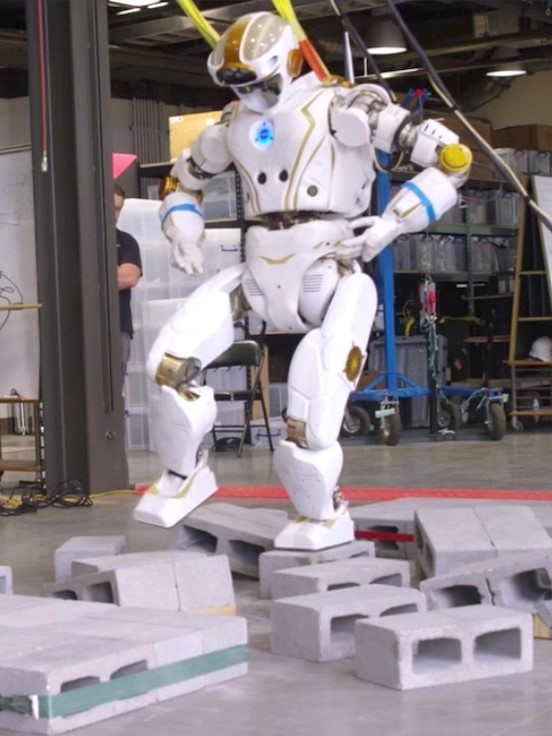
\includegraphics[width=.8\linewidth]{STYLESTUFF/Valkyrie.jpeg}
    \caption{}
     \label{fig:currentrobotsc}
  \end{subfigure}
   \begin{subfigure}{0.23\textwidth}
     \centering
  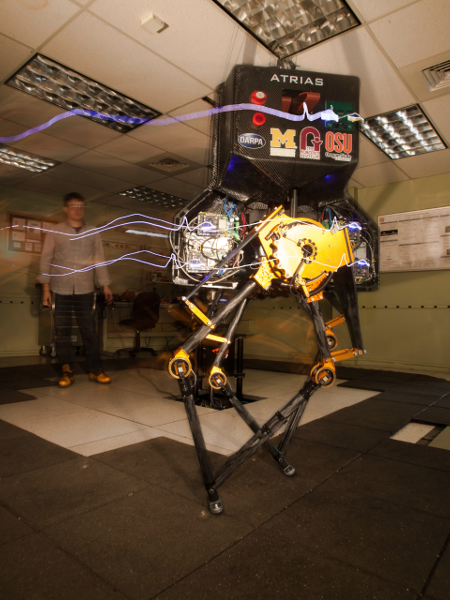
\includegraphics[width=.8\linewidth]{STYLESTUFF/ATRIAS.png}
  \caption{}
   \label{fig:currentrobotsd}
  \end{subfigure}
  \caption{A selection of currently popular humanoid robots. \textbf{(a)} Boston Dynamics' new Atlas \cite{newatlas}. \textbf{(b)} Previous version of Atlas \cite{oldatlas} and \textbf{(c)} NASA's Valkryie \cite{valkyrie} walking over rough terrain at IHMC. \textbf{(d)} ATRIAS, a bipedal robot \cite{atrias}.}
  \label{fig:currentrobots}
\end{figure}
\subsection{Modeling}
As can be seen from the images in \figref{fig:currentrobots}, a lot of bipedal robots are capable of more tasks than walking alone. As this survey is focused on walking and stabilizing by the legs, tasks as for example grasping and having environment contact of the upper body are not considered. However, even without contact the upper body plays a crucial roll in the dynamics of the robot. Chest and arm movements can create angular momentum that can control the system, which is considered in this survey. An example of the modeling of a full robot in joints and links can be found in \cite{yamaguchi1999development}.\\
\subsection{Simulation}
Because of the complexity and size of the systems considered, simulation is key. There exist multiple simulation environments, from which one of them is the open source Gazebo \cite{koenig2004design}. At IHMC an inhouse developed simulation environment is used: \ac{SCS}. This environment is written in Java.

\section{\ac{LIP} Models}
In modeling of walking, one of the most important assumptions often made is the modeling of the stance leg as a \ac{LIP}, as for example in \cite{kajita20013d}. Besides this, a not-linearized inverted pendulum is also widely used in the modeling of walking \cite{kuo2005energetic}. For planning and control however, a linearized description is desirable. In the \ac{2D} \ac{LIP} equations of motion
\begin{equation}
\ddot{x}=\frac{g}{l}x
\label{eq:LIPeom}
\end{equation}
where $l$ is the pendulum length and $x$ the Cartesian x-coordinate of the pendulum tip, the motion of the tip along the x-axis does not affect $l$. At any position $x$, a local virtual straight pendulum can be considered, so this motion is at a constant height and $l=z_0$  holds. As in \ac{3D} by the linear model the system dynamics can be decoupled, the dynamics in $y$-direction will read the same: $\ddot{y}=\frac{g}{l} y$. In \figref{fig:3dlip} this motion is visualized if the \ac{CoM} is relatively far from from the base. The pendulum base lies in the origin and $\boldsymbol{x} = [x,y]^T$ is the \ac{2D} \ac{CoM} projection on the horizontal plane. Because the \ac{LIP} assumption holds, the vertical component of the leg force $\boldsymbol{f}$ has to cancel out gravity acceleration: $f_z=mg$.
\begin{figure}[h]
\centering
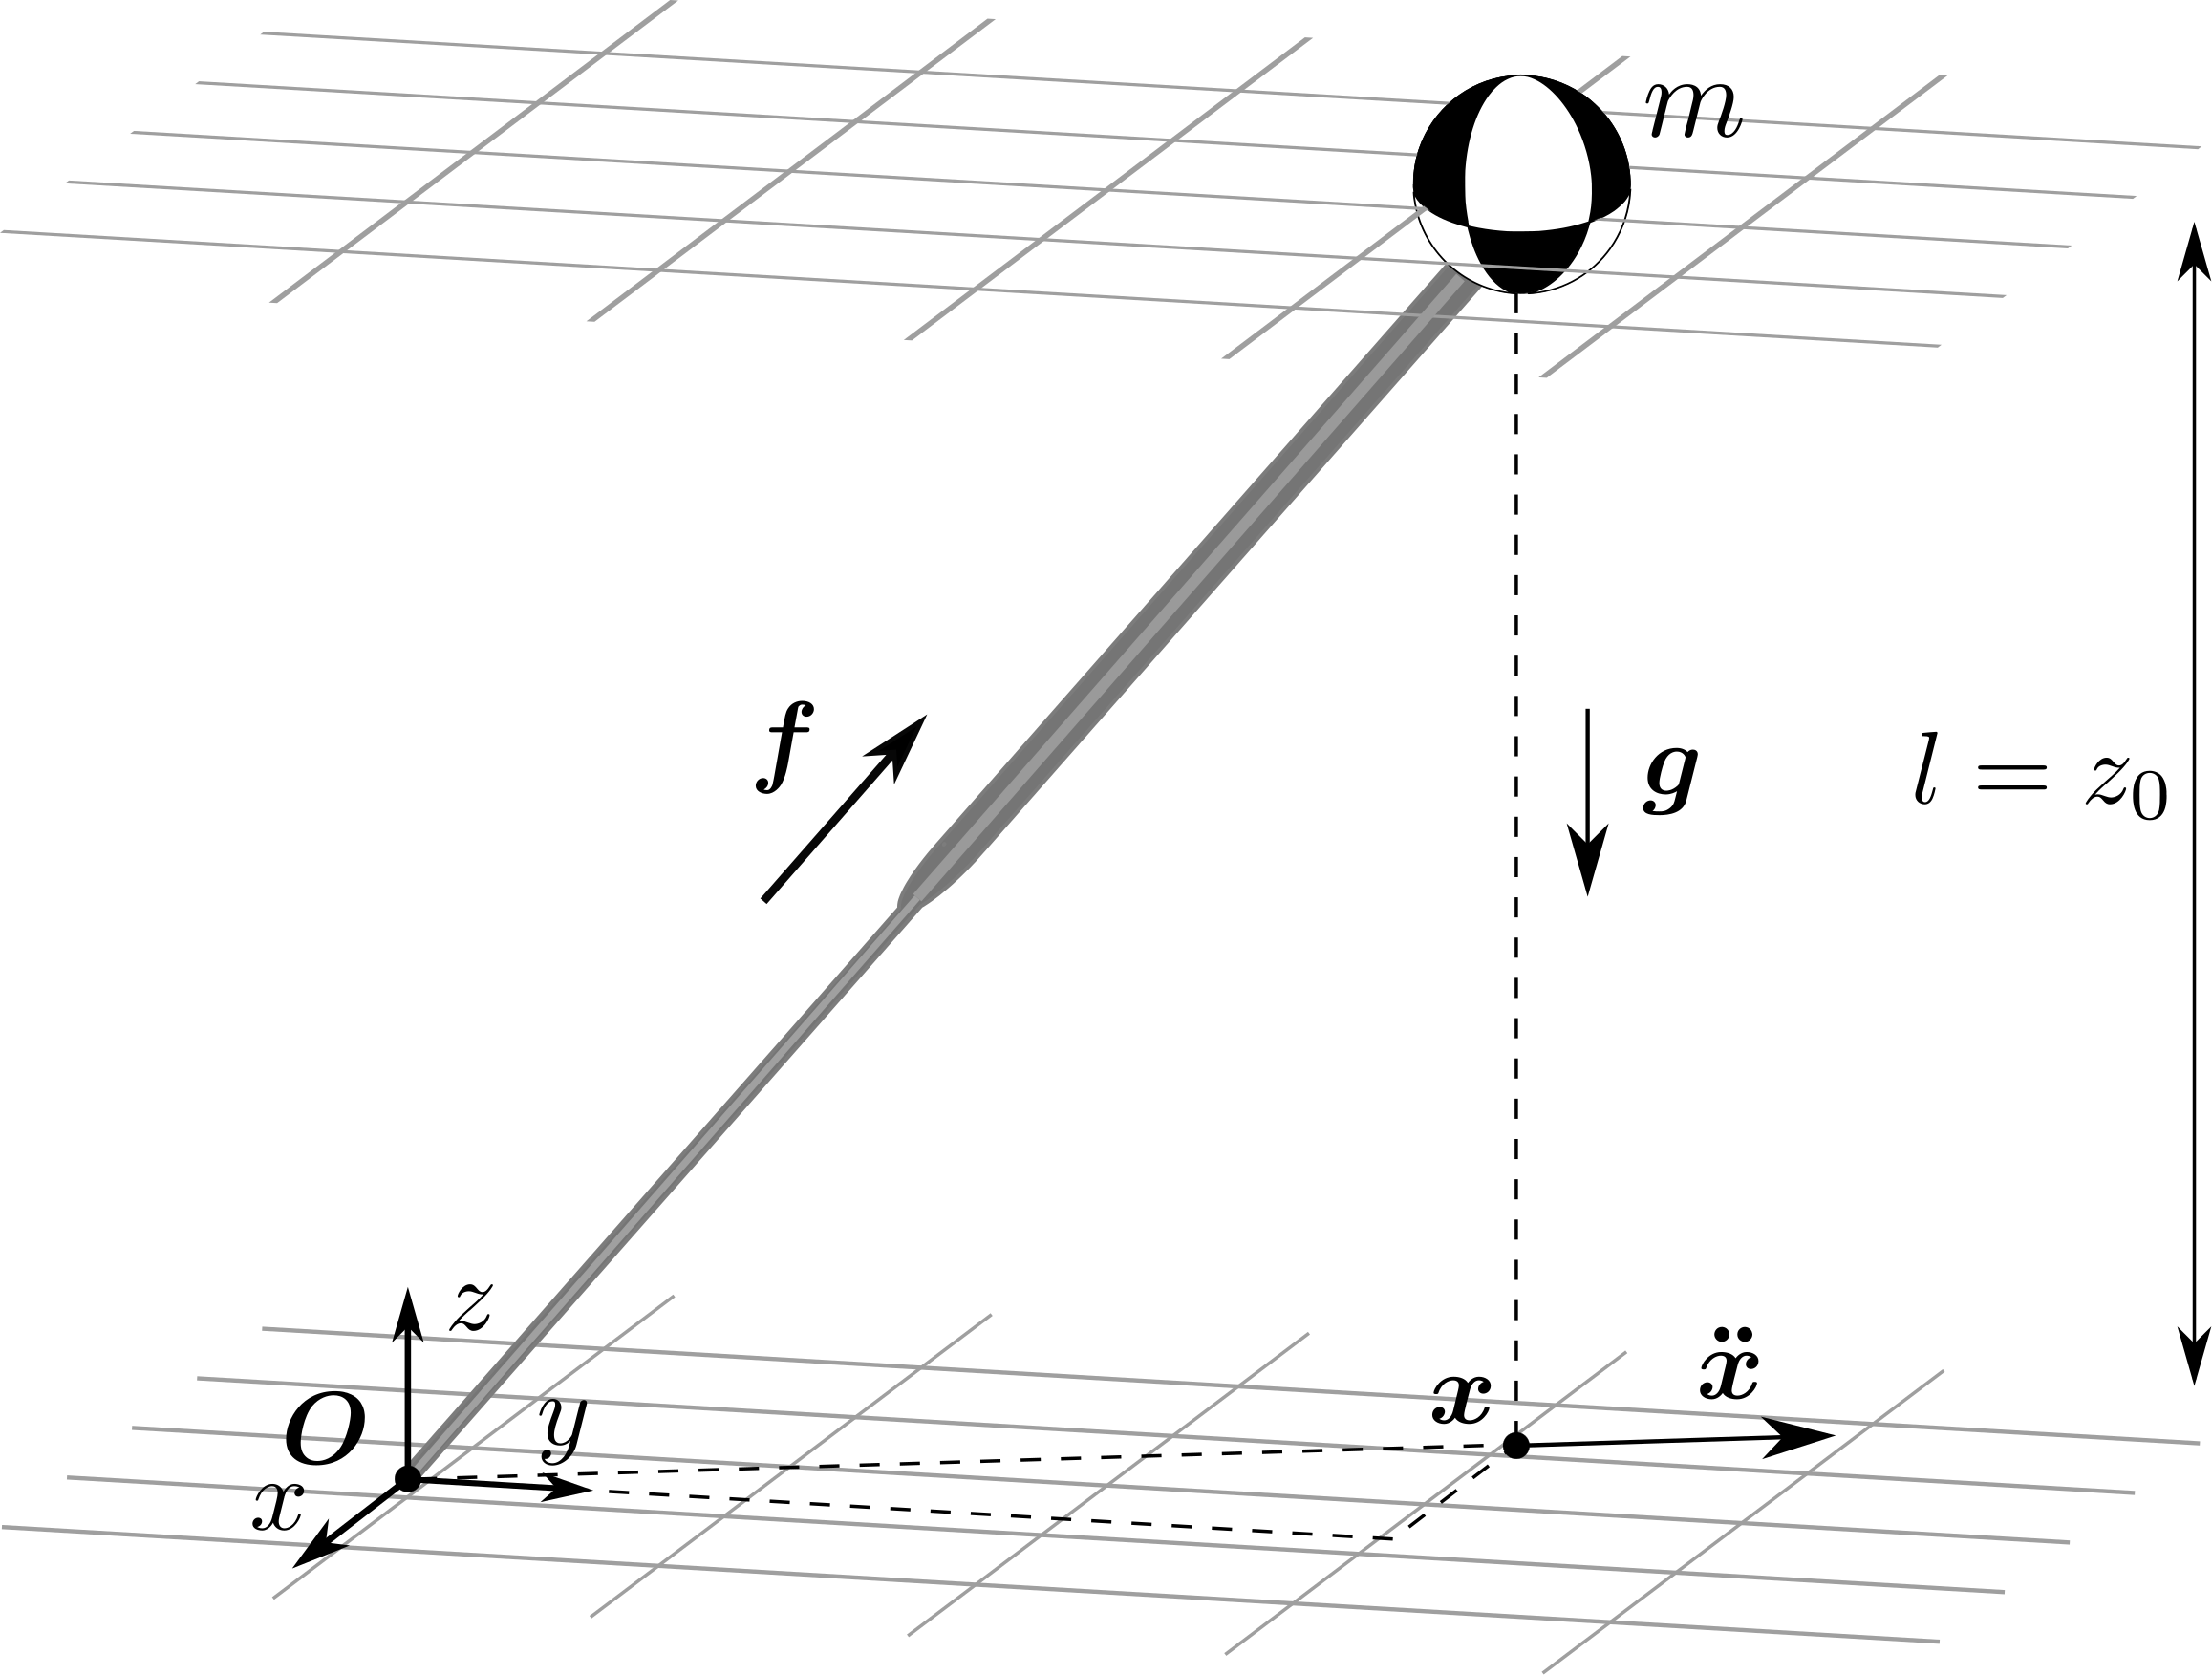
\includegraphics[width=0.5\textwidth]{STYLESTUFF/3DCoMwithoutfoot.png}
\caption{\ac{3D} motion of \ac{LIP} model.}
\label{fig:3dlip}
\end{figure}

\subsection{Conservation of \ac{Elip}}
\cite{kajita1992dynamic} had a crucial finding in an extended use of \ac{LIP} models. Because $F=ma$, $I=Fv$ and $E = Fs = \int Fv dt$, there can be reasoned that if one takes the time integral of the product of the second and the first derivative of a state, an expression for a normalized energy can be achieved: $\frac{E}{m}=\int av dt$. In the mentioned publication that same action is applied on Eq. \eqref{eq:LIPeom}:
\begin{equation}
\int (\ddot{x}-\frac{g}{l}x)\dot{x} dt = \frac{1}{2}\dot{x}^2-\frac{g}{2z_0}x +C=0
\label{eq:Elip}
\end{equation}
with $C$ the integration constant. The \ac{LIP} Orbital Energy is defined as $E_{LIP}=-C$. 

\subsection{The \acf{ICP}}
Although the finding of the \ac{LIP} Orbital Energy was very important for future robot motion modeling, more than a decade later \cite{pratt2006capture} introduced the \ac{CP}. Taking $E_{LIP}=0$ and taking the square root of Eq.  \eqref{eq:Elip} gives
\begin{equation}
x_{CP}=\sqrt{ \frac{z_0}{g}}\dot{x} 
\label{eq:cp}
\end{equation}
where $x_{CP}$ is the \ac{CP}, measured from the current pendulum tip position, based on the current tip velocity $\dot{x}$. This is the point where the velocity is driven to zero and the pendulum is upright. In \figref{fig:2dicp} a \ac{2D} visual explanation is given of this point.
\begin{figure}[h]
\centering
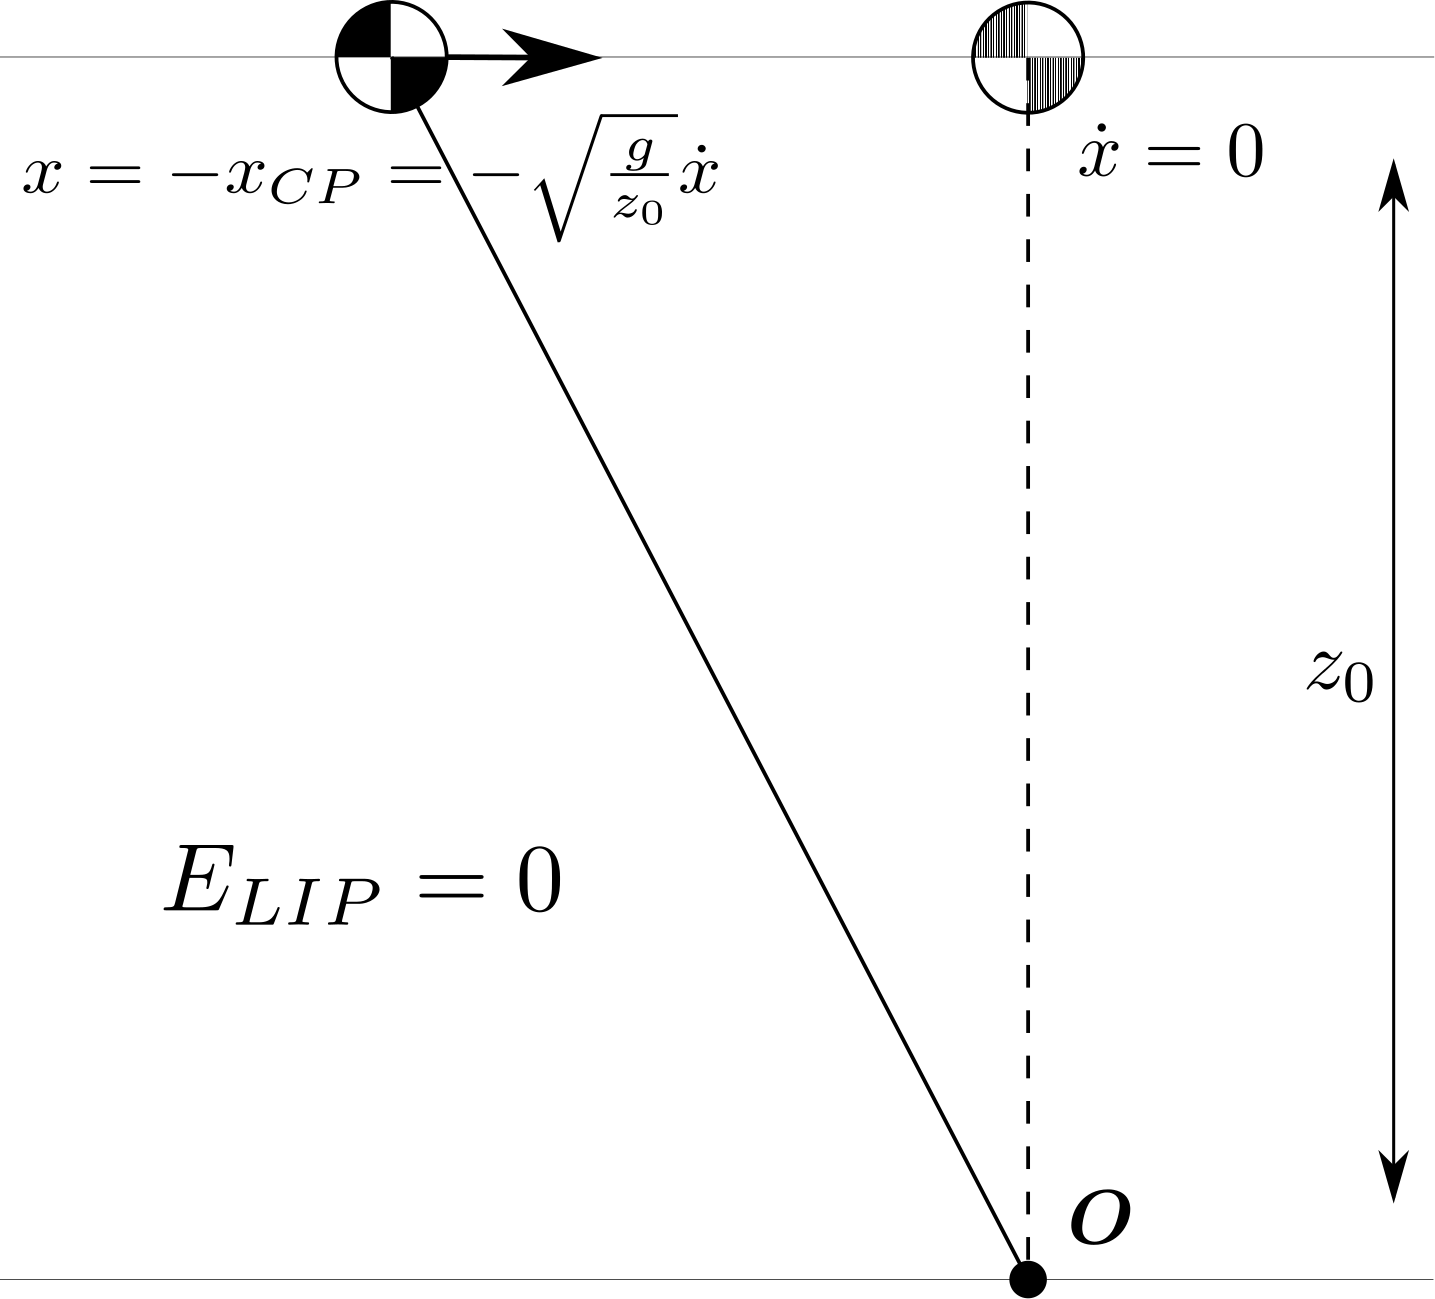
\includegraphics[width=0.4\textwidth]{STYLESTUFF/2DICP.png}
\caption{Visualization of path and states by the capture of the point mass according \ac{ICP} theory.}
\label{fig:2dicp}
\end{figure}
Later, the \ac{ICP} was introduced \cite{koolen2012capturability}, which gives a slightly different discription of the point:
\begin{equation}
x_{ICP}=x+\sqrt{ \frac{z_0}{g}}\dot{x} 
\label{eq:icp}
\end{equation}
where $x_{ICP}$ is the \ac{ICP}. In this way, the point can be described in the environment coordinates.
The $x$- and $y$ coordinate can be decoupled as in the equation of motion of Eq. \eqref{eq:LIPeom}. However, in the \ac{2D} horizontal plane it is not guaranteed that the velocity direction of the \ac{CoM} is towards the ankle point. 
\subsubsection{\ac{ICP} dynamics}
Because the ankle is not always located at the same location as the \ac{ICP} for the current horizontal velocity, for modeling and planning the time derivative is taken of the \ac{ICP}, which is named the \ac{ICP} dynamics \cite{koolen2012capturability}. This time derivative can be written as a function of the current \ac{ICP} location:
\begin{equation}
\boldsymbol{\dot{x}}_{ICP}=\sqrt{ \frac{g}{z_0}}\boldsymbol{x}_{ICP} 
\label{eq:cp}
\end{equation}
where $\boldsymbol{x}_{ICP}$ is the $xy$-vector of the \ac{ICP} location and assuming that the pendulum base is the origin.

\section{Humanoid Robot Terminology}
As the \ac{ICP} is a measure for the behavior of a bipedal robot, there exist plenty of terms and descriptions for specific virtual points and forces on and acting on the robot. In this section a short summary is given from the most popular jargon.

\subsection{The \ac{CoP}}
The larger feet of a human than those of a dog make him more capable of upright walking, due to an increase of controllability of the modeled-as-\ac{LIP} human. The ankles can apply a torque that would virtually move the position of the base of the inverted pendulum, so that the linear acceleration on the \ac{CoM} as in Eq. \eqref{eq:LIPeom} and the capture point as in Eq. \eqref{eq:cp} change. The new virtual base is called the \ac{CoP}. By its definition, this point only lives within the foot polygon \cite{vukobratovic2004zero}. In \figref{fig:3dlipfoot} the definition of the \ac{CoP} is visualized. If the point mass is restricted to move on a constant height, the vertical component of $\boldsymbol{f'}$ counteracts gravity: $f'_z=g$. 
\begin{figure}[h]
\centering
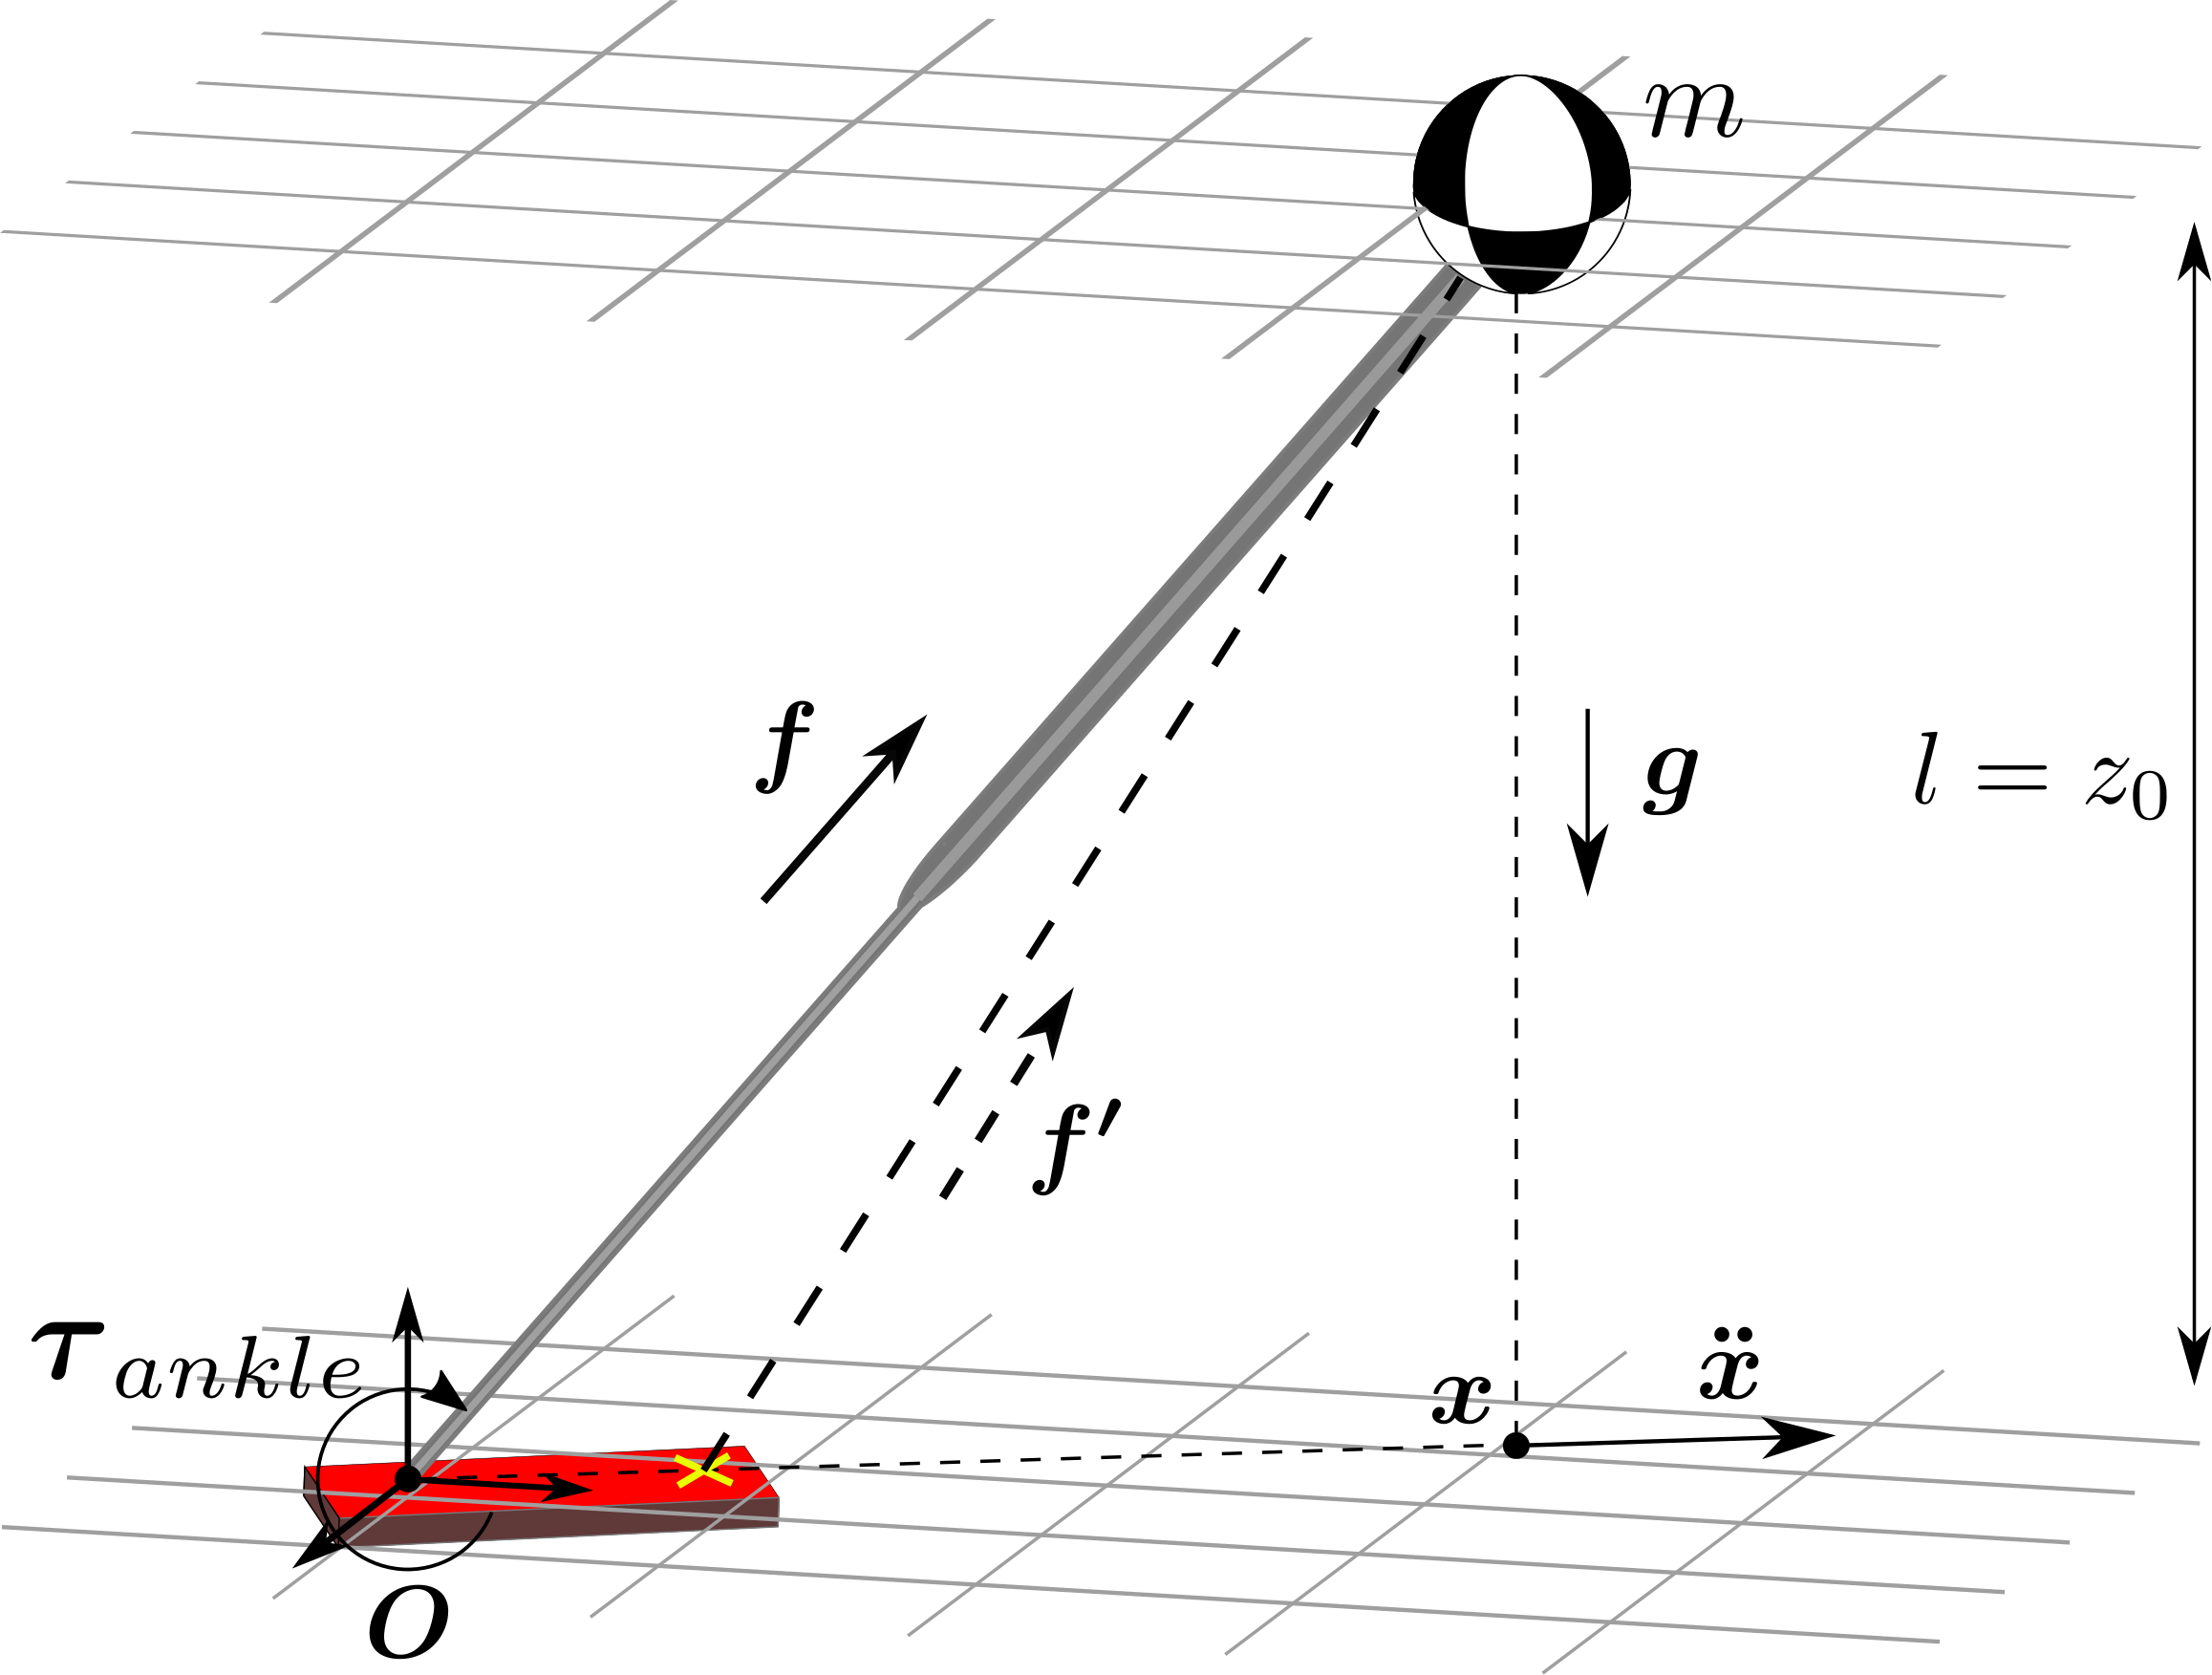
\includegraphics[width=0.5\textwidth]{STYLESTUFF/3DCoMwithfoot.png}
\caption{\ac{3D} motion of \ac{LIP} model with foot. The yellow cross points out the \ac{CoP} location.}
\label{fig:3dlipfoot}
\end{figure}

\subsection{The \ac{ZMP}}
The \ac{ZMP} coincides during stable walking with the \ac{CoP}, like described in \cite{vukobratovic2004zero}. The two points however are not equal in unstable or more complicated cases, like falling over.  The \ac{CoP} is restricted to be in the foot polygon, as this is a point that links to contact forces \cite{sardain2004forces}. The \ac{ZMP} however is not restricted to lie within the foot polygon. The \ac{ZMP} is the point on the ground where the tipping moment equals zero. The tipping moment is defined as the component of the moment that is tangential to the ground surface. The \ac{ZMP} initially was introduced in \cite{vukobratovic1969contribution}.

\subsection{The \ac{CMP}}
The earlier mentioned points give sufficient measure for a \ac{LIP} model with point mass and finite sized feet. However, any angular momentum applied by the body does not affect those points. In the case of the \ac{CoP} for example, the model assumes the resulting reacting force acts from the \ac{CoP} through the \ac{CoM} The \ac{CMP} takes angular momentum into account, which can be used as a measure and for control \cite{popovic2005ground}. This is defined as the point where a line passing through the \ac{CoM}, parallel to the ground reaction force intersects with the ground surface. The \ac{CMP} is defined as
\begin{eqnarray}
x_{CMP} = x_{ZMP} + \frac{\tau_{y,CoM}}{F_{gr,z}}\\
y_{CMP} = y_{ZMP} - \frac{\tau_{x,CoM}}{F_{gr,z}}
\end{eqnarray}
where $\tau_{CoM}$ is the torque around the \ac{CoM}, $[x_{ZMP},y_{ZMP}]$ the \ac{ZMP} location on the horizontal plane and $F_{gr,z}$ is the ground reaction force in z-direction in Cartesian space. In \figref{fig:3dlipfootinertia} it is displayed how the body angular momentum affects the ground reaction force $\boldsymbol{f'}$ from the \ac{CoP} and how the \ac{CMP} can be determined with the intersection of a parallel line through the \ac{CoM} and the ground plane. For clarity the point in the image lies on the line from $\boldsymbol{O}$ to $\boldsymbol{x}$. This has not to be the case however, as the body can exert angular momentum along all axes. 
\begin{figure}[h]
\centering
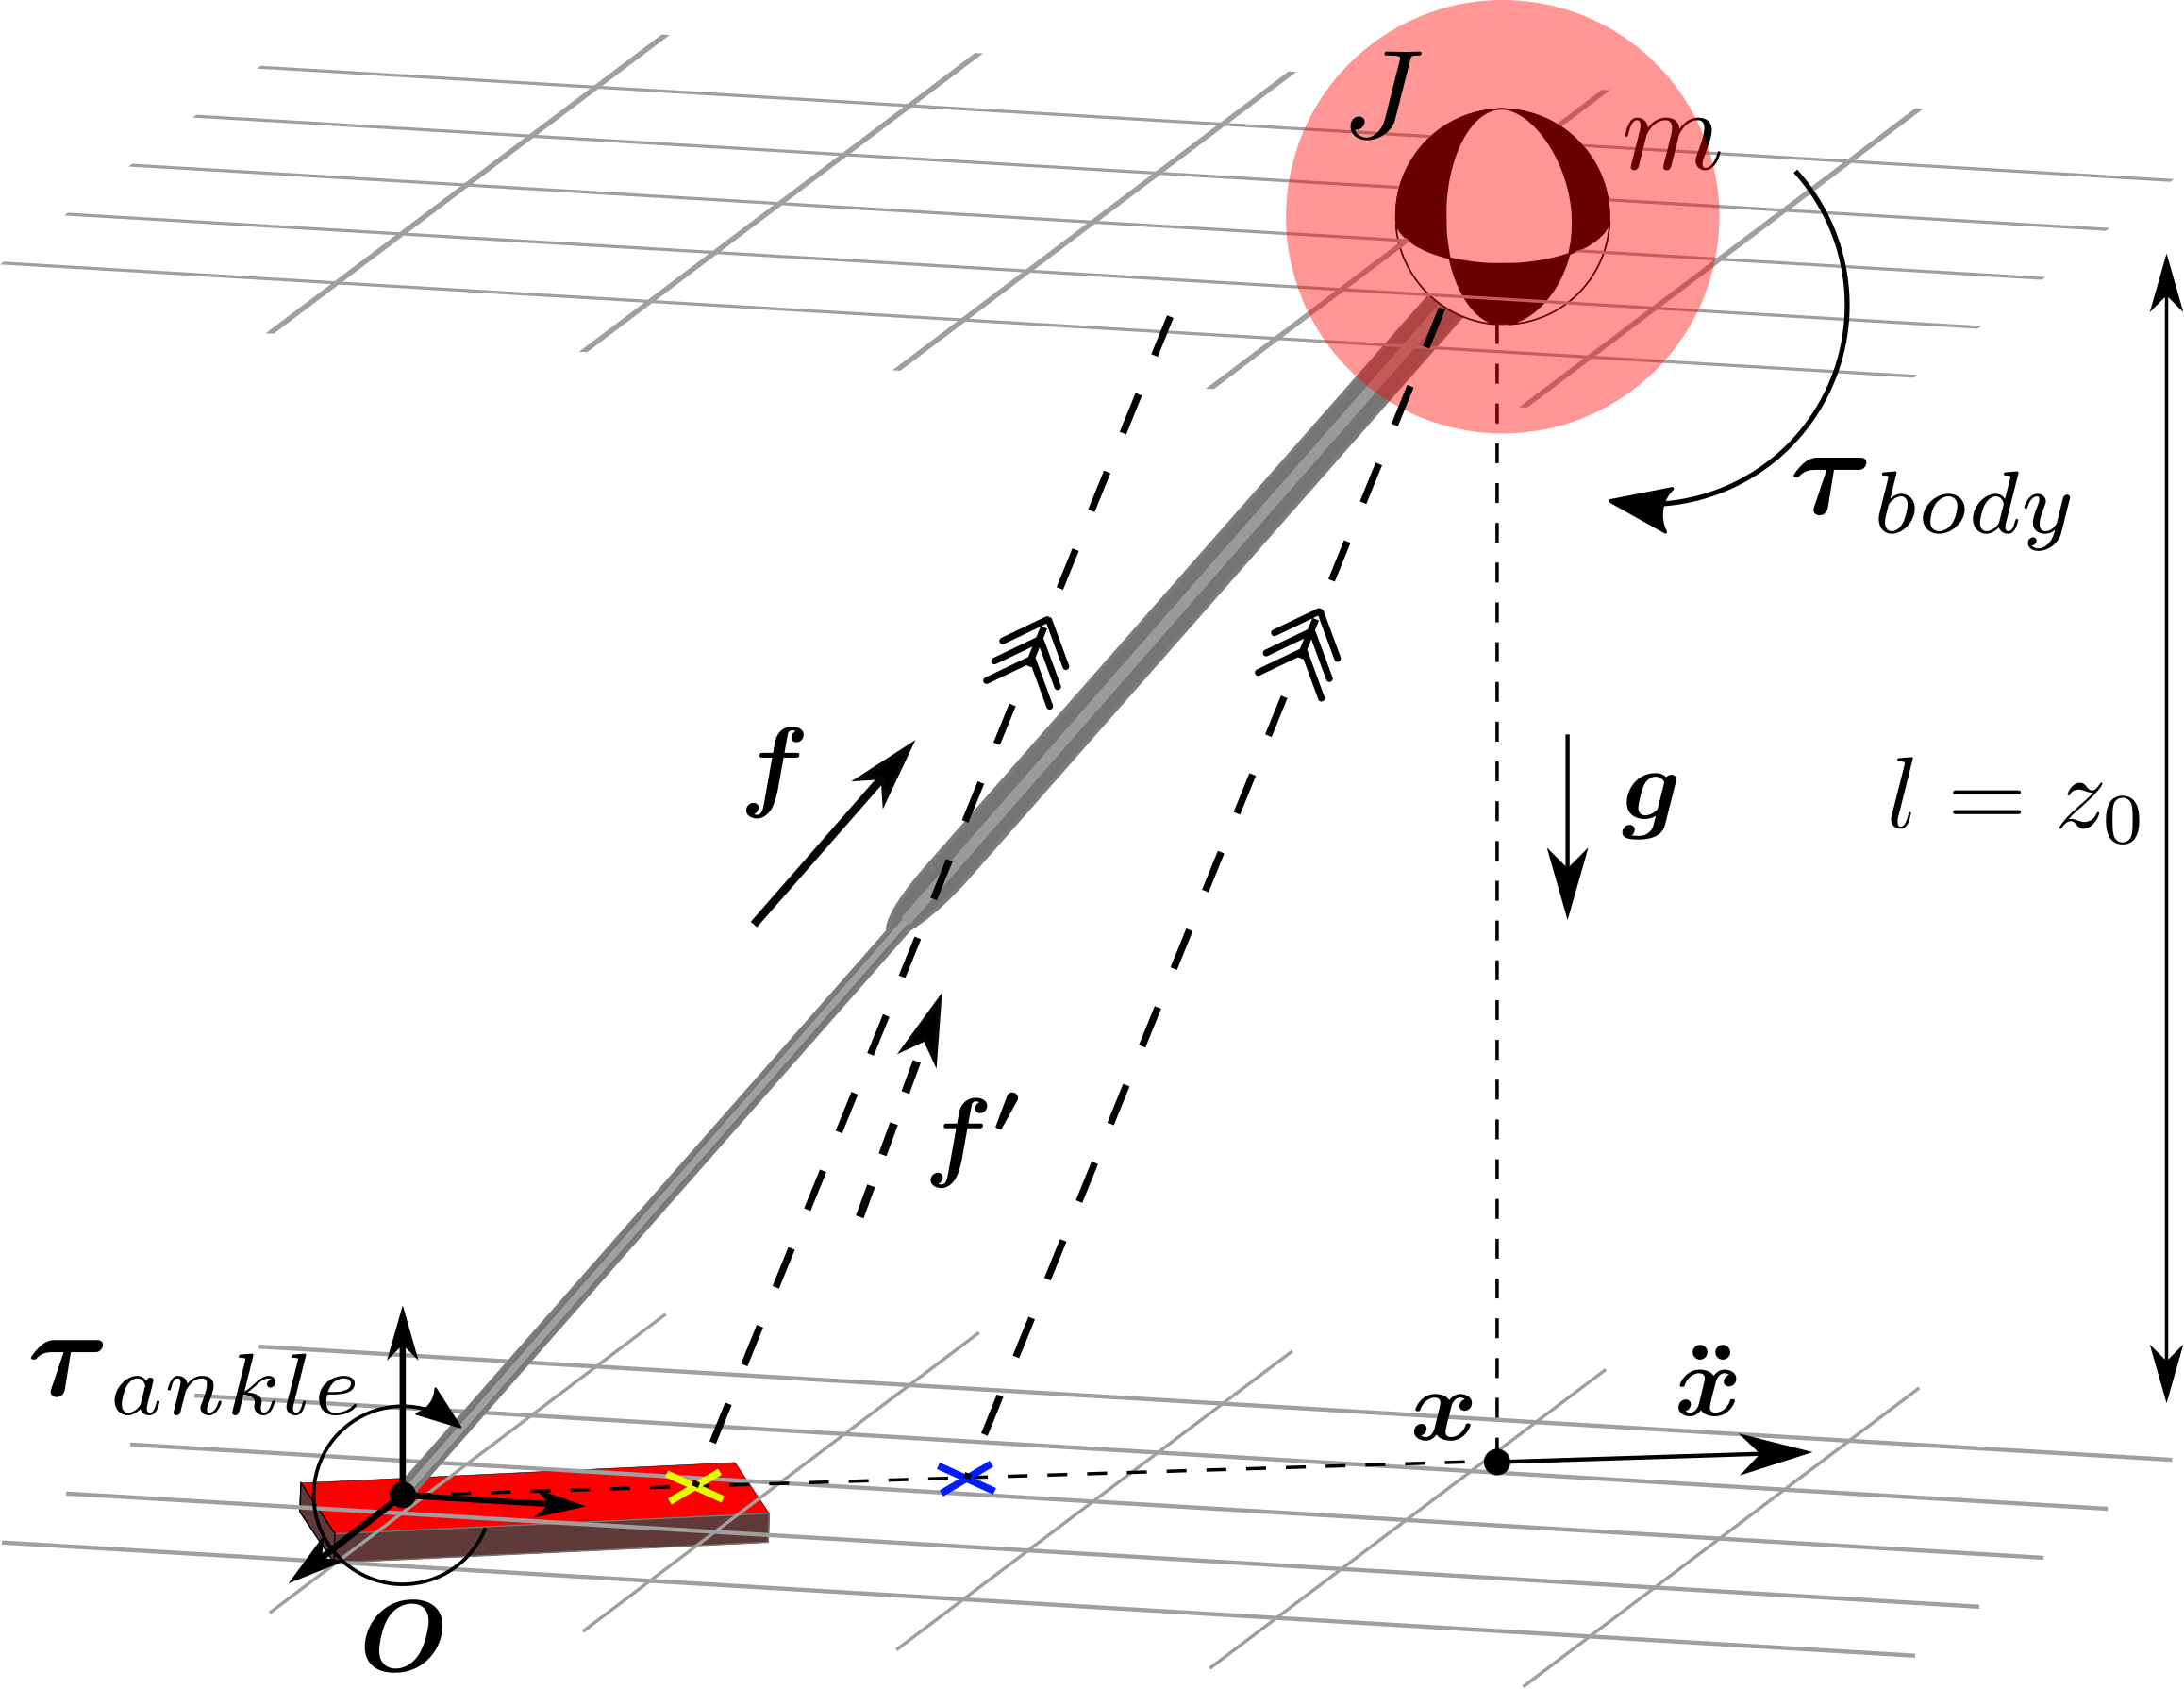
\includegraphics[width=0.5\textwidth]{STYLESTUFF/3DCoMwithfootinertia.png}
\caption{\ac{3D} motion of \ac{LIP} model with foot and body inertia. The blue cross points out the \ac{CMP} location.}
\label{fig:3dlipfootinertia}
\end{figure}
\subsection{Linear momentum rate}
To combine the effects described in this section in one single measure, often the linear momentum or linear momentum rate is considered in the horizontal plane. This boils down to be a combination of the \ac{LIP} equations of motion and the \ac{CoP}, \ac{ZMP} or \ac{CMP}. Using the \ac{CMP} the linear momentum rate is then defined as
\begin{equation}
\boldsymbol{\dot{l}} = m\boldsymbol{\ddot{x}}= m\frac{g}{z}(\boldsymbol{x}-\boldsymbol{x}_{CMP})
\label{eq:ldot}
\end{equation}
where $\boldsymbol{\dot{l}}$ is the linear momentum rate in the horizontal plane, $\boldsymbol{x}$ the \ac{2D} \ac{CoM} position and $\boldsymbol{x}_{CMP}$ the \ac{CMP} position.
\subsection{Other points}
Other than the points mentioned before, there are sometimes other points considered in humanoid robotics. Examples of this are the \ac{eCMP} and the \ac{VRP} \cite{englsberger2013three}, but those are not further discussed here. 

\section{Analysis \& Discussion}
From the study in this chapter it becomes clear that oftentimes the complex system of a walking robot is captured in a relatively simple model, namely that of a \ac{LIP} with a mass with inertia on the tip and a base that is maneuverable within limits. The combined dynamics of this configuration define the dynamics in the horizontal plane of the \ac{LIP}. This however requires the nominal ground reaction force to have a vertical component equal to the force applied by gravity. For motion over a flat surface, it seems intuitively as a desirable goal to have a constant height. If the goal is to move somewhere in the planar world, height variation and thus height acceleration would only waste energy. However, for having a walking motion where the gravity vector is not perpendicular to it, the assumption of the constant force in vertical direction might not be a solid assumption. Even on a flat surface the \ac{CoM} varies slightly in height \cite{lee1998determinants}. Moreover, varying leg force could be used to accelerate or stop quicker, which would mean a different force is applied than assumed in the \ac{LIP} model. The different leg force changes the horizontal component of the force, which can control the motion. This also results in a change of its vertical component, which after time changes the \ac{CoM} height, as it is not equal to gravitational forces anymore.